
\chapter{Fundamentação Teórica}
\label{fundamentacao-teorica}

\section{Geomarketing}
O Geomarketing pode ser entendido como uma ferramenta de análise estatística de dados, com intuito de localizar padrões que possam ser utilizados e combinados na elaboracao de indicadores, perfis de consumo e estrategias de negócios, de modo a auxiliar na tomada de decisões. Geralmente, o servico é oferecido por consultorias especializadas - o  objetivo da empresa que contratante é a melhoria no desempenho de seu negócio.

O Geomarketing é ainda pouco difundido no Brasil, no entanto cada vez mais se populariza no âmbito dos negócios: segundo \cite{Exame}, utilizado de forma amadora há 20 anos, o uso de ferramentas de localização geográfica evoluiu e alcançou importância dentro da estratégia de expansão das empresas: grupos como Coca-Cola e O Boticário usam o marketing geográfico e pequenas e médias empresas já começam a mirar em sistemas de busca com foco na geolocalização.

\section{Ferrametas de contagem de pessoas}
Ferramentas de contagens de pessoas são sistemas eletrônicos que utilizam leitores para contar as pessoas \cite{trafsysdef}. A contagem de pessoas
num determinado período resulta no tráfego de indivíduos. Esta informação quando aliada com outras métricas de negócio proporciona a gestores
informações estratégicas.

Não existe apenas um método para contar o número de pessoas. As principais diferenças entre os contadores estão: área de cobertura, densidade e tecnologia utilizada. Os principais
métodos de contagem são:
\begin{itemize}
  \item \textbf{Feixes infravermelhos:}são colocados na entrada de lojas emitindo um feixe infravermelho entre os seus extremos, quando
  alguém interrompe o feixe, uma entrada é contada. A área de cobertura é pequena e a densidade de pessoas que ele permite passando pela porta
  ao mesmo tempo é baixíssima;
  \item \textbf{Imagens térmica:} o uso de sensores térmicos e processamento de imagens para distinguir a quantidade de pessoas. Normalmente, são
  posicionados no teto para que a imagem capture a temperatura no topo da cabeça dos indivíduos.
\end{itemize}




\section{Trabalhos correlatos}
Este subcapítulo apresenta algumas soluções que empregam o tráfego de usuários como técnica de \emph{geomarketing}.

\subsection{Cidade Jardim}
A Zebra Technologies é uma empresa internacional líder em fornecer serviços e soluções que permitem às organizações observarem suas operações em
tempo real. As áreas de atuação da empresa se diversificam: saúde,
transporte e logística, inteligência, localização e \emph{e-commerce}. Como soluções, a empresa oferece produtos
que utilizam tecnologias, como: RFID, computadores móveis, leitor de código de barras,
quiosques interativos, software, impressoras, entre outros. Já serviços, a Zebra oferece planejamento e execução de projetos para identificação
e rastreamento computadorizado.

Em 2016, a empresa implantou no Shopping Cidade Jardim em São Paulo o seu projeto MPact. Este oferece a clientes acesso gratuito à Internet,
que quando conectados, consegue a localização do consumidor em três níves: zona, posição e presença. Com estas informações, é possível saber
sobre uma determinada pessoa: quem é, onde está, quanto tempo fica em certas áreas e quais produtos está adquirindo. Utilizando a rede Wi-Fi e
Bluetooth, este projeto identifica a posição e o tempo exato onde cada consumidor se encontra.

O MPact proporciona aos varejistas, lojistas e operadores do shopping melhor entendimento sobre o comportamento dos consumidores. Por exemplo, é
possível saber quais corredores estão mais cheios, quais lojas estão vendendo mais e quais pontos mais chamam a atenção, ou seja, este sistema
auxilia no monitoramento de pontos de venda. Segundo a \citeonline{zebra} esta é uma maneira de entender o que os clientes querem,
para então ganhá-los e mantê-los.

\subsection{Meshlium Xtreme}
O Meshlium Xtreme é um produto da empresa Libelium que detecta dispositivos móveis e veículos para garantir inteligência de negócios. Ao detectar dispositivos
através de sinais Wi-Fi e Bluetooth, esse sistema mede pessoas e carros, gerando informações \cite{libelium}. Sobre a atividade de pessoas as informações
são: quantidade
de pessoas passando numa rua diariamente, média de tempo que as pessoas ficam numa rua, diferença entre visitantes e residentes e rotas
de caminhadas pelas lojas. Sobre veículos: número de veículos em tempo real passando em certo ponto, média de tempo que veículo fica parado,
média de velocidade e tempos de viagem em rotas alternativas quando congestionamento é detectado.

Através de sinais Wifi e Bluetooth, os dispositivos detectados não precisam estar conectados a nenhum AP, possibilitando a detecção de qualquer um
independente da fabricante. Já veículos são detectados até 100 km/h. O objetivo principal dete produto é medir a quantidade de pessoas e carros
num determinado ponto e uma hora específica, permitindo que sejam tomadas decisões estratégicas sobre o tráfego de pessoas e carros sobre área.
As figuras \autoref{meshlium-celulares} e \autoref{meshlium-carros} demonstram o funcionamento do produto.

\begin{figure}[htb]
	\caption{\label{meshlium-celulares}Detecção de \emph{smartphones}}
	\begin{center}
		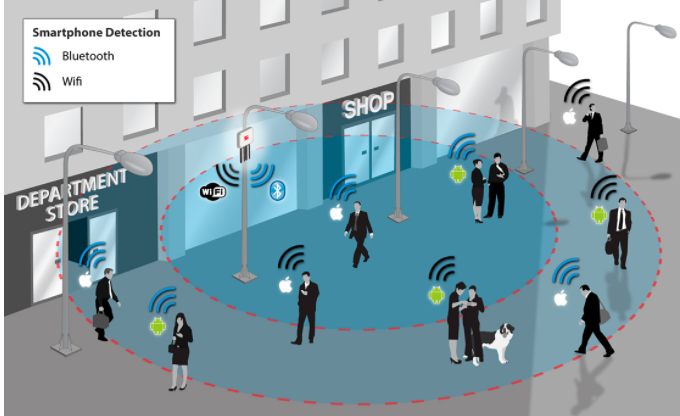
\includegraphics[width=0.70\textwidth]{img/meshlium-celulares.png}
	\end{center}
	\legend{Fonte: \cite{libelium}.}
\end{figure}

\begin{figure}[htb]
	\caption{\label{meshlium-carros}Detecção de veículos}
	\begin{center}
		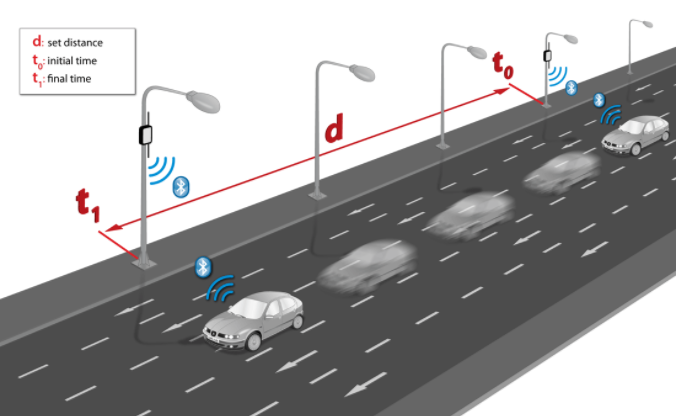
\includegraphics[width=0.70\textwidth]{img/meshlium-carros.png}
	\end{center}
	\legend{Fonte: \cite{libelium}.}
\end{figure}
